\documentclass[12pt,a4paper]{report}
\usepackage[utf8]{inputenc}
\usepackage{amsfonts}
\usepackage{amssymb}
\usepackage{graphicx}
\usepackage{float}

% sets margin
\usepackage[hmargin=3cm,vmargin=2.5cm]{geometry}

% creates landscape pages
\usepackage{pdflscape}

% defining settings for textpost
\usepackage[absolute]{textpos}
\setlength{\TPHorizModule}{\paperwidth}
\setlength{\TPVertModule}{\paperheight}

% headers / footers
\usepackage{fancyhdr}
\pagestyle{fancy}
\fancyhf{}
\rhead{Assignment 1a}
\lhead{CSG1132: Communicating in an IT Environment}
\rfoot{\thepage}
\lfoot{Martin Ponce, ID: 10371381}
\renewcommand{\footrulewidth}{0.5pt}

% defining landscape headers / footers
\fancypagestyle{fancylscape}{
	\fancyhf{}
	\renewcommand{\footrulewidth}{0pt}
	\renewcommand{\headrulewidth}{0pt}
	% header
	\begin{textblock}{0.05}[-0.5,-2](0,0)
		{\rotatebox{90}{CSG1132: Communicating in an IT Environment}}
	\end{textblock}
		\begin{textblock}{0.05}[-0.5,-1](0,0)
		{\rotatebox{90}{Assignment 1a}}
	\end{textblock}
	\begin{textblock}{0.05}[-1,-0.109](0,0)
		{\rotatebox{90}{\rule{24.2cm}{0.5pt}}}
	\end{textblock}
	% footer
	\begin{textblock}{0.05}[-19,-4.28](0,0)
		{\rotatebox{90}{Martin Ponce, ID: 10371381}}
	\end{textblock}
		\begin{textblock}{0.05}[-19,-12.8](0,0)
		{\rotatebox{90}{\thepage}}
	\end{textblock}
		\begin{textblock}{0.05}[-18.7,-0.109](0,0)
		{\rotatebox{90}{\rule{24.2cm}{0.5pt}}}
	\end{textblock}
}

% adjusts padding between caption and figure
\setlength{\belowcaptionskip}{20pt}

% adds links to references and colors them blue
\usepackage{hyperref}
\hypersetup{colorlinks=true,
			linkcolor=blue,
			citecolor=blue,
			urlcolor=blue}

% apa style referencing
\usepackage[sectionbib, natbibapa]{apacite}
\usepackage{chbibref}

% front matter
\title{Edith Cowan University\\CSG1132\\Communicating in an IT Environment\\Assignment 1a}
\author{Concept Map, Thesis Statements \& Learner Reflection\\\\
		Martin Ponce\\Student 10371381\\Tutor: Dr. Mark Brogan}
\date{August 24, 2014}

\begin{document}

% title page
\maketitle

% toc
\makeatletter
\tableofcontents

\newpage
\section*{\textsf{Task 1: Concept Map}}
\addcontentsline{toc}{section}{Task 1: Concept Map}

\subsection*{\textsf{Focus Question:}}
What is the role of psychology in personal use of Facebook?\\

See \emph{Figure 1.}

\subsection*{\textsf{Concept Map Reference List}}
\begin{itemize}
\item \citet*{Pai2013}
\item \citet*{McAndrew2012}
\item \citet*{Nadkarni2012}
\item \citet*{Moore2012}
\item \citet*{Ross2009}
\item \citet*{Toma2013}
\item \citet*{Ellison2007}
\item \citet*{Park2011}
\item \citet*{Anderson2012}
\item \citet*{Ku2013}
\item \citet*{Rosen2013}
\item \citet*{Trottier2012}
\item \citet*{Kwan2013}
\end{itemize}

\newpage
\newgeometry{hmargin=3cm,vmargin=2.5cm}
\thispagestyle{fancylscape}
\begin{landscape}
\begin{figure}[H]
	\centering
	\caption{Concept map}
	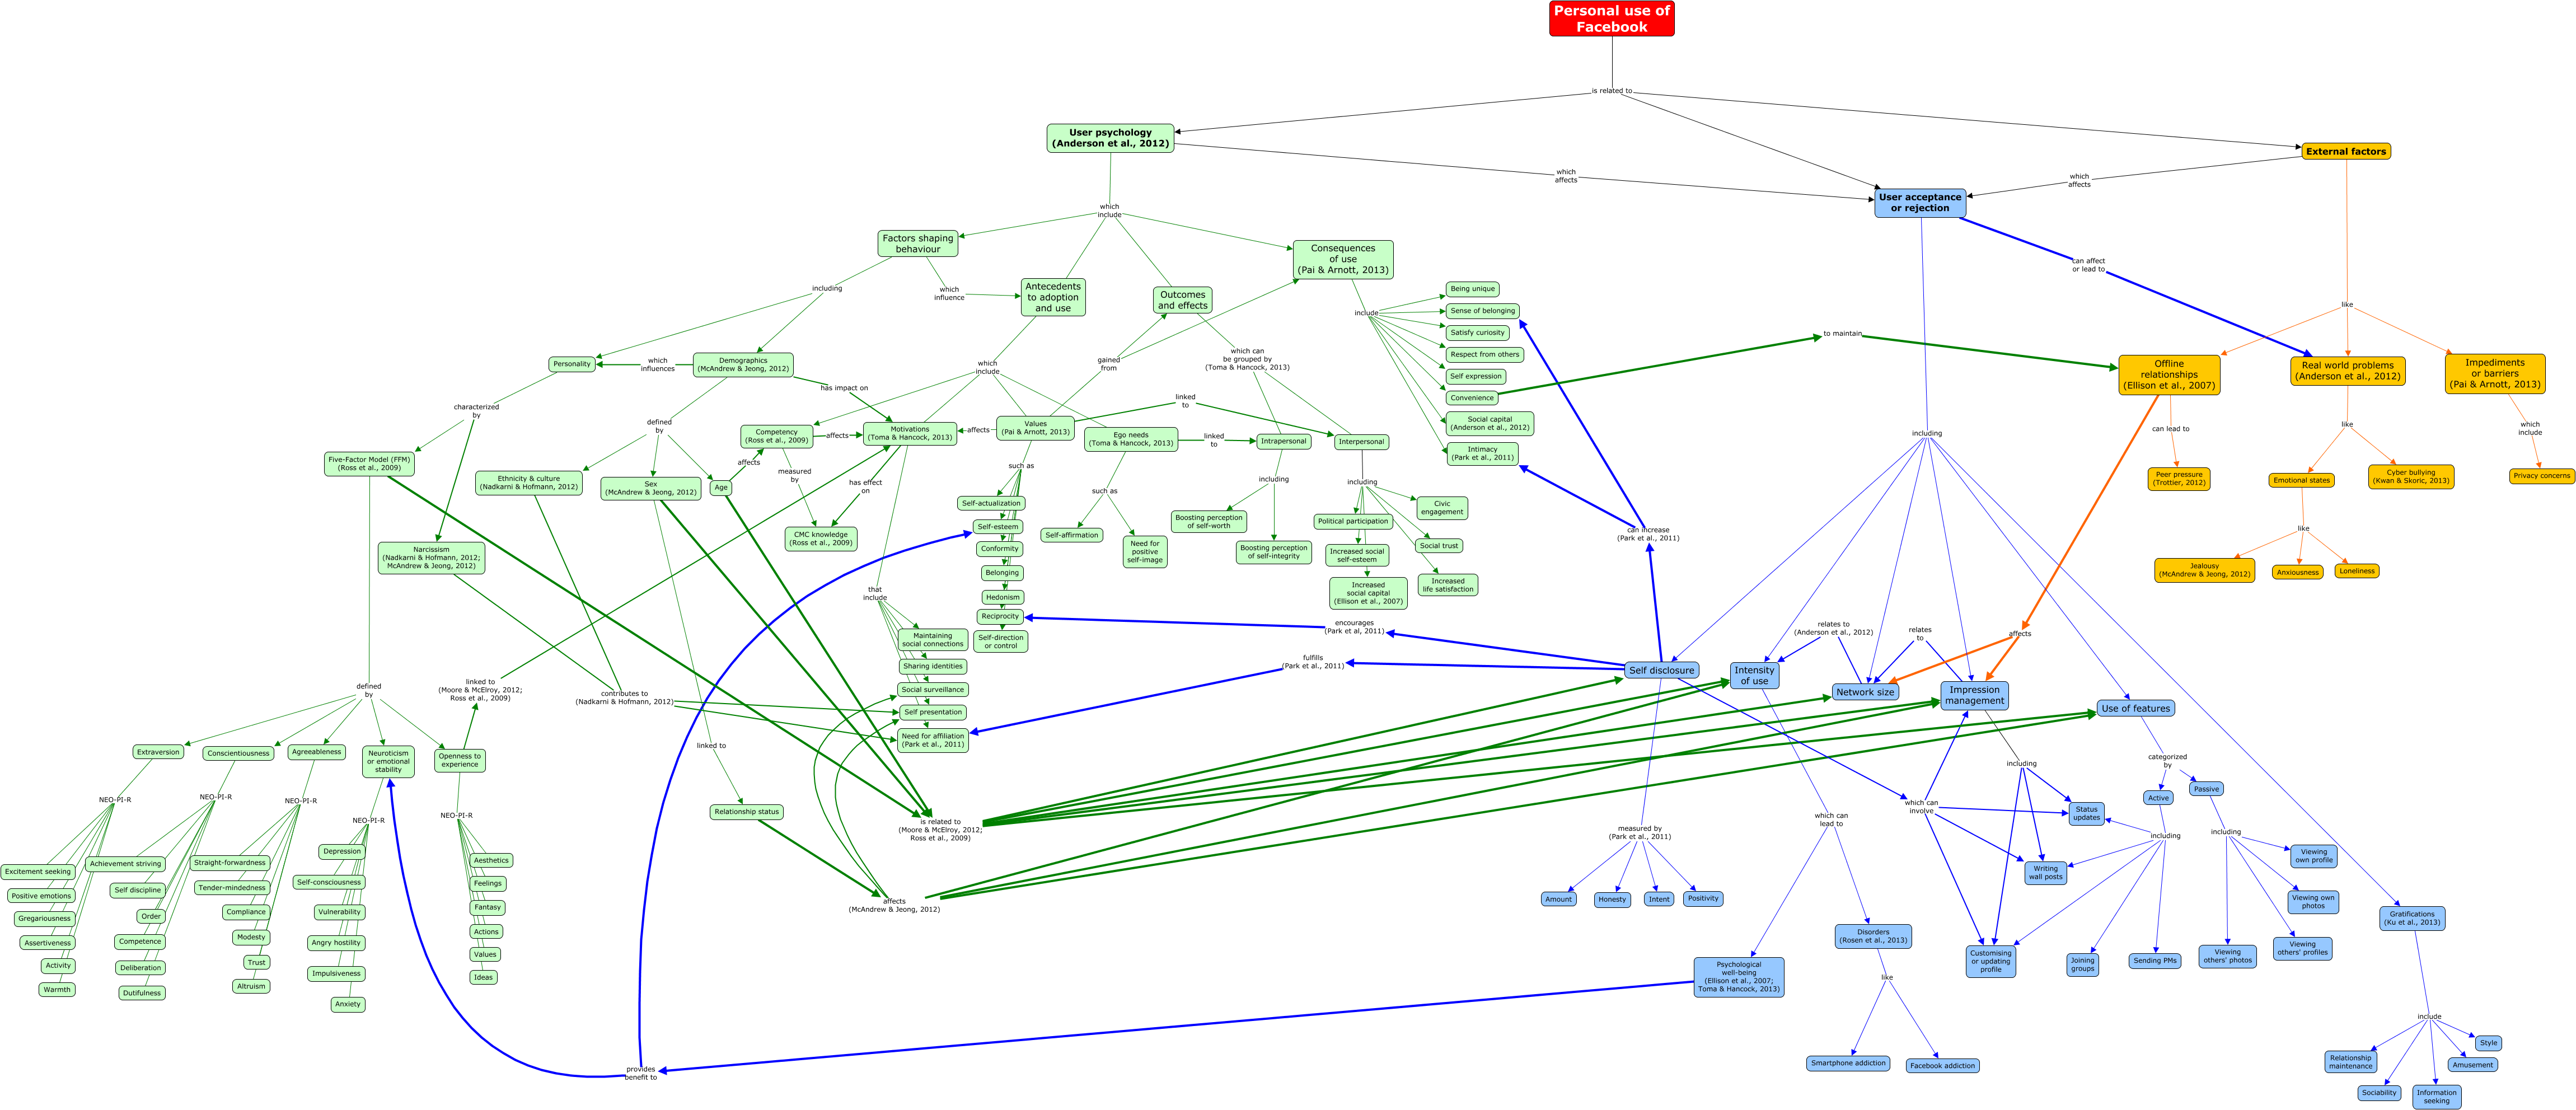
\includegraphics[scale=0.16]{./img/CSG1132_Facebook_Cmap_v9.png}
\end{figure}
\end{landscape}
\restoregeometry

\newpage
\section*{\textsf{Task 2: Thesis Statements}}
\addcontentsline{toc}{section}{Task 2: Thesis Statements}

\subsection*{\textsf{Argumentative Statement}}

\subsubsection*{\textsf{Question:}}

Can a user's relationship status affect their usage of Facebook? \citep{McAndrew2012}.

\subsubsection*{\textsf{Statement Development:}}
\begin{enumerate}
\item The relationship status: Modifying user behaviour on Facebook.
\item A user's relationship status as a behaviour modifier on Facebook.
\item The relationship status as a predicator of Facebook use.
\item The relationship status impacts user behaviour on Facebook.
\end{enumerate}

\subsection*{\textsf{Analysis Statement}}

\subsubsection*{\textsf{Question:}}
What are the motivations for self-disclosure on Facebook? \citep{Park2011}.

\subsubsection*{\textsf{Statement Development:}}
\begin{enumerate}
\item Self-disclosure on Facebook fulfils the human need for affiliation.
\item Facebook self-disclosure and it's relation to the human need for affiliation.
\end{enumerate}

\subsection*{\textsf{Exposition Statement}}

\subsubsection*{\textsf{Question:}}
What are the psychological benefits in the use of Facebook? \citep{Toma2013}.

\subsubsection*{\textsf{Statement Development:}}
\begin{enumerate}
\item The positive psychological effects of Facebook use.
\item The positive psychological effects of Facebook use are increased perceptions of self-worth and self-integrity.
\end{enumerate}

\newpage
\section*{\textsf{Task 3: Summary \& Learner Reflection}}
\addcontentsline{toc}{section}{Task 3: Summary \& Learner Reflection}

\subsection*{\textsf{Concept Map Summary}}
\addcontentsline{toc}{subsection}{Concept Map Summary}
The concept map was developed in 1972 by researchers at Cornell Univesity and is used as a tool to visually organise and present knowledge, usually in reference to a focus question or topic \citep{Novak2006, Hilbert2009}. \citet[pp. 267]{Hilbert2009} explains that concept mapping is ``based on Ausebel's assimilation theory of cognitive learning''. A concept map consists of a collection of concepts that relate to a particular subject or problem domain, and are written inside bubbles or `nodes' which are then linked together with lines to display their associations with one another. Unlike mind maps, these lines are labelled to express the relationships between these linked concepts, otherwise referred to as ``path labelling'' by \citet[pp. 790]{Rodriguez-Priego2013}.\\

Concept maps are structured in a hierarchical sense, where the most general concepts are displayed at the top of the map, and more specific, less inclusive concepts are drawn towards the bottom of the map \citep{Novak2006}. Another characteristic of a concept map is its non-linearity. Concept maps have the ability to `cross-link' and display relationships between concepts in separate domains within the given topic. Such cross-links demonstrates that the researcher has developed a deeper understanding of the topic, has created new understanding through the research, and is able to express relationships and propositions between outlying concepts that may have not been immediately evident prior to research \citep{Novak2006}. This method is in contrast to a mind map where such flexibility or specificity is not required to be expressed, and concepts are only linked to their direct counterparts without the ability to label identified relationships explicitly.\\

According to \citet[pp.1]{Novak2006}, a concept map ``serves as a kind of \emph{template} or \emph{scaffold} to help organize knowledge and to structure it''. It is due to this structure that concept maps may be used to define the scope of the topic to be researched and assists in identifying knowledge gaps in domains where further research could be gathered \citep{Novak2006}. As stated previously, concept maps display information in an organised, non-linear manner which allows for scalablility so that new concepts can be logically connected to pre-existing nodes and assists in organising information as they are found during research \citep{Novak2006}. Concept maps facilitate in the organisation of information gathered from study or research from many sources in a coherent and flexible manner which makes it a valued tool for learning.

\newpage
\subsection*{\textsf{Learning Reflection}}
\addcontentsline{toc}{subsection}{Learning Reflection}
As I enrolled for university as a first year, undergraduate student, one of my main concerns was academic writing. I understood that this was something I would be expected to do and was concerned about my ability to perform in this area. Concept mapping has helped me break down the overwhelming amount of information from peer-reviewed journal articles into smaller digestible pieces and make sense of the information I was taking in.\\

After getting a grasp of the topic at hand, I developed a sense of which documents would become valuable for the assignment by scanning the abstracts to determine if the article is relevant to my research. This allowed me to cut down my quickly growing reading list.\\

As I began to develop the concept map, I found it difficult to organise the information in any kind of hierarchy and started my way from the bottom, with the most specific concepts. This resulted in concept maps that seemed more like mind maps. I found \citet{Novak2006} ``The Theory Underlying Concept Maps and How To Construct and Use Them'' a valuable resource and used the methods outlined in the article. In particular, I found the \emph{parking lot} method the most useful, dropping concepts into the map as I was reading articles, and then deciding on their associations after I finished reading and developed a better understanding of the relationships between the concepts.\\

Once a good structure and foundation for the concept map was established, it was easier to identify cross-links between different concepts. The difficult part was deciding which cross-links were most important, and deciding how to present these links with so many lines intersecting and overlapping each other. This resulted in many iterations of the map, while I attempted to arrange concepts in a hierarchical sense while accommodating for these cross-links.\\

Completing the second assignment task, which involved writing thesis statements based on articles, provided a different view and helped identify even more cross-links from the articles. Completing this exercise also highlighted the most important cross-links and has motivated me to redesign the concept map once more to emphasise those links.\\

As a student, I believe concept mapping is a great tool and appreciate its value when used correctly for academic writing. It helps make sense of information that come from a variety of sources and assists in identifying/generating new ideas. I have started using the tool for other units, and find it particularly useful for a systems analysis assignment, where there are many moving parts and concept mapping allowed me to get a broad overview of the system before making decisions. I understand there are formal ways of modelling a system, but the concept map allowed me to visualise and understand the system very quickly with specific detail without having to learn any particular modelling methodology first. I look forward to more opportunities where I can use concept maps and truly appreciate being introduced to this wonderful tool for learning.

\newpage
\urlstyle{rm}
\setbibref{\textsf{References}}
\bibliographystyle{apacite}
\addcontentsline{toc}{section}{References}
\bibliography{./bib/bib}

\end{document}